\documentclass[12pt,a4paper]{article}
\usepackage[utf8]{inputenc}
\usepackage[russian]{babel}
\usepackage[OT1]{fontenc}
\usepackage{amsmath}
\usepackage{amsfonts}
\usepackage{amssymb}
\usepackage{graphicx}
\usepackage{wrapfig}
\usepackage[left=2cm,right=2cm,top=2cm,bottom=2cm]{geometry}
\author{Николай Козырский}
\title{Лабораторная работа № 1.1 \\
		 Экспериментальная проверка уравнения Эйнштейна для фотоэффекта и определение постоянной планка}
\begin{document}
\maketitle
\section{Теория}
Фотоэффект -- испускание электронов фотокатодом, облучаемым светом -- хорошо объясняется фотонной теорией света: фотон с энергией $ \hbar \omega $ выбивает электрон с поверхности металла и сообщает электрону кинетическую энергию.

Энергетический баланс этого взаимодействия описывается уравнением:
\begin{equation} \label{energy}
\hbar \omega = W + E_{max},
\end{equation}
где $W$ -- работа выхода электрона из катода, $E_{max}$ -- максимальная кинетическая энергия электрона после выхода из фотокатода.



Для измерения энергии вылетевших фотоэлектронов вблизи фотокатода обычно располагается второй электрод, на который подается задерживающий ($V < 0$) или ускоряющий ($V > 0$) потенциал. При достаточно больших ускоряющих напряжениях фототок достигает насыщения (рис. \ref{curdep}): все испущенные электроны попадают на анод. При задерживающих потенциалах на анод попоадают лишь электроны, обладающие достаточно большой кинетической энергией, в то время как медленно движущиеся электроны заворачиваются полем и возвращаются на катод. При некотором значении $V = -V_0$ (потенциал запирания) даже наиболее быстрые фотоэлектроны не могут достичь анода. 

Максимальная кинетическая энергия $E_{max}$ электронов связана с запирающим потенциалом $V_0$ соотношением $E_{max} = e V_0$. Подставляя это соотношение в равенство (\ref{energy}), мы получаем уравнение Эйнштейна для фотоэффекта:
\begin{equation} \label{einstein}
e V_0 = \hbar \omega - W
\end{equation}

Чтобы определить величину запирающего напряжения, нам надо правильно экстраполировать получаемую токовую зависимость к нулю, т.е. определить, какова функциональная зависимость $I(V)$. Расчет для простейшей геометрии -- плоский катод, освещаемый светом, и параллельный ему анод -- приводит к зависимости 
\begin{equation} \label{Idep}
\sqrt{I} \propto (V_0 - V).
\end{equation}

Для экспериментальной проверки уравнения Эйнштейна по графикам $ \sqrt{I} = f(V)$ определяются потенциалы запирания  $V_0$ при разных частотах и строится зависимость $V_0(\omega)$, которая, как следует из (\ref{einstein}), должна иметь вид
\begin{equation}
V_0(\omega) = \frac{ \hbar \omega - W}{e}.
\end{equation}

По наклону этой прямой можно определить постоянную Планка:
\begin{equation}
\frac{dV_0}{d\omega} = \frac{\hbar}{e}
\end{equation}

\section{Экспериментальная установка}

\begin{wrapfigure}{r}{0.5\linewidth} \label{scheme} 
%\vspace{-5ex}  
 \center{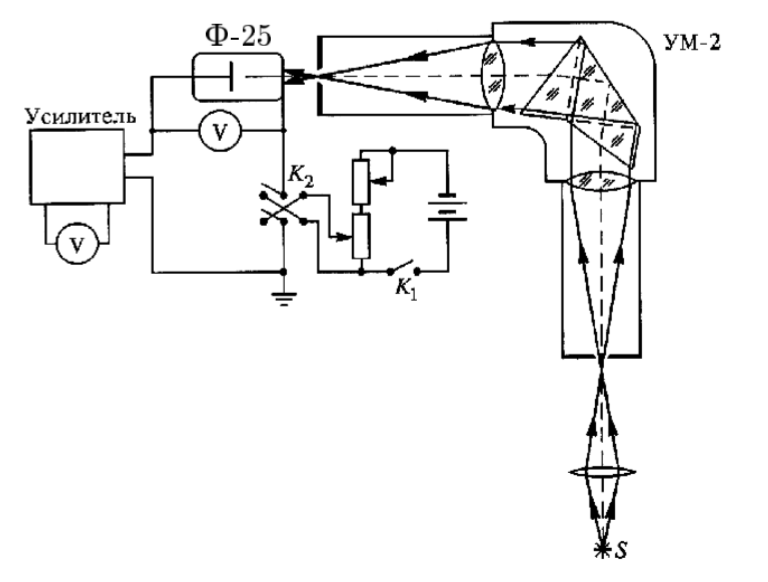
\includegraphics[width=.7\linewidth]{scheme.png}}
\caption{Схема установки}
\end{wrapfigure}

Схема установки приведена на рис. \ref{scheme}. Свет от источника S с помощью конденсора фокусируется на входную щель монохроматора УМ-2, выделяющего узкий спектральный интервал, и попадает на катод фотоэлемента Ф-25. 

\section{Ход работы}

\begin{enumerate}
\item Проградуировать шкалу монохроматора с помощью неоновой лампы 
\item Для 4-5 длин волн измерить зависимость $I(V)$
\end{enumerate}

\section{Обработка полученных результатов}

\begin{enumerate}
\item Градуировка монохроматора:

\begin{figure}[h]
 \center{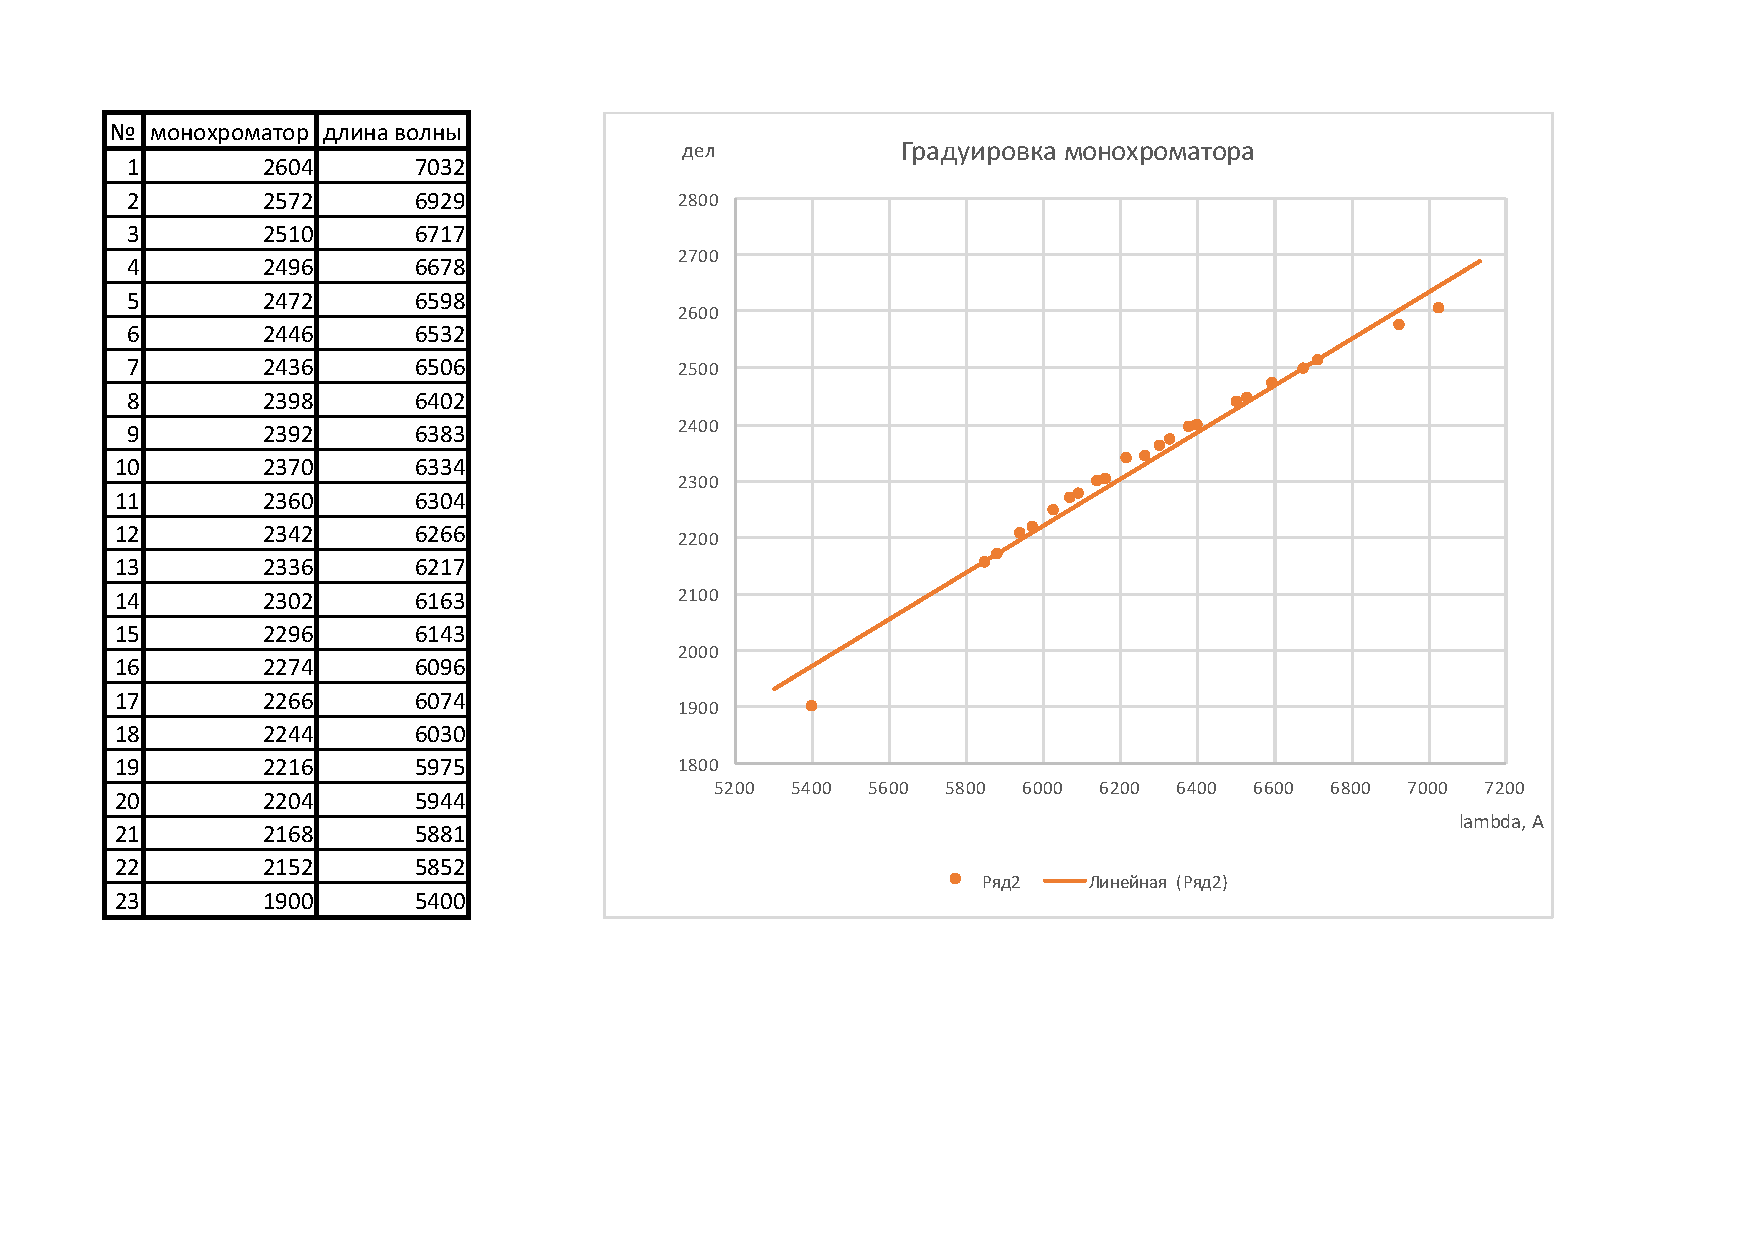
\includegraphics[width=.8\linewidth]{lab1.pdf}}
\end{figure}

\newpage

\item Измерение $V_0( \omega)$:

\begin{figure}[h]
 \center{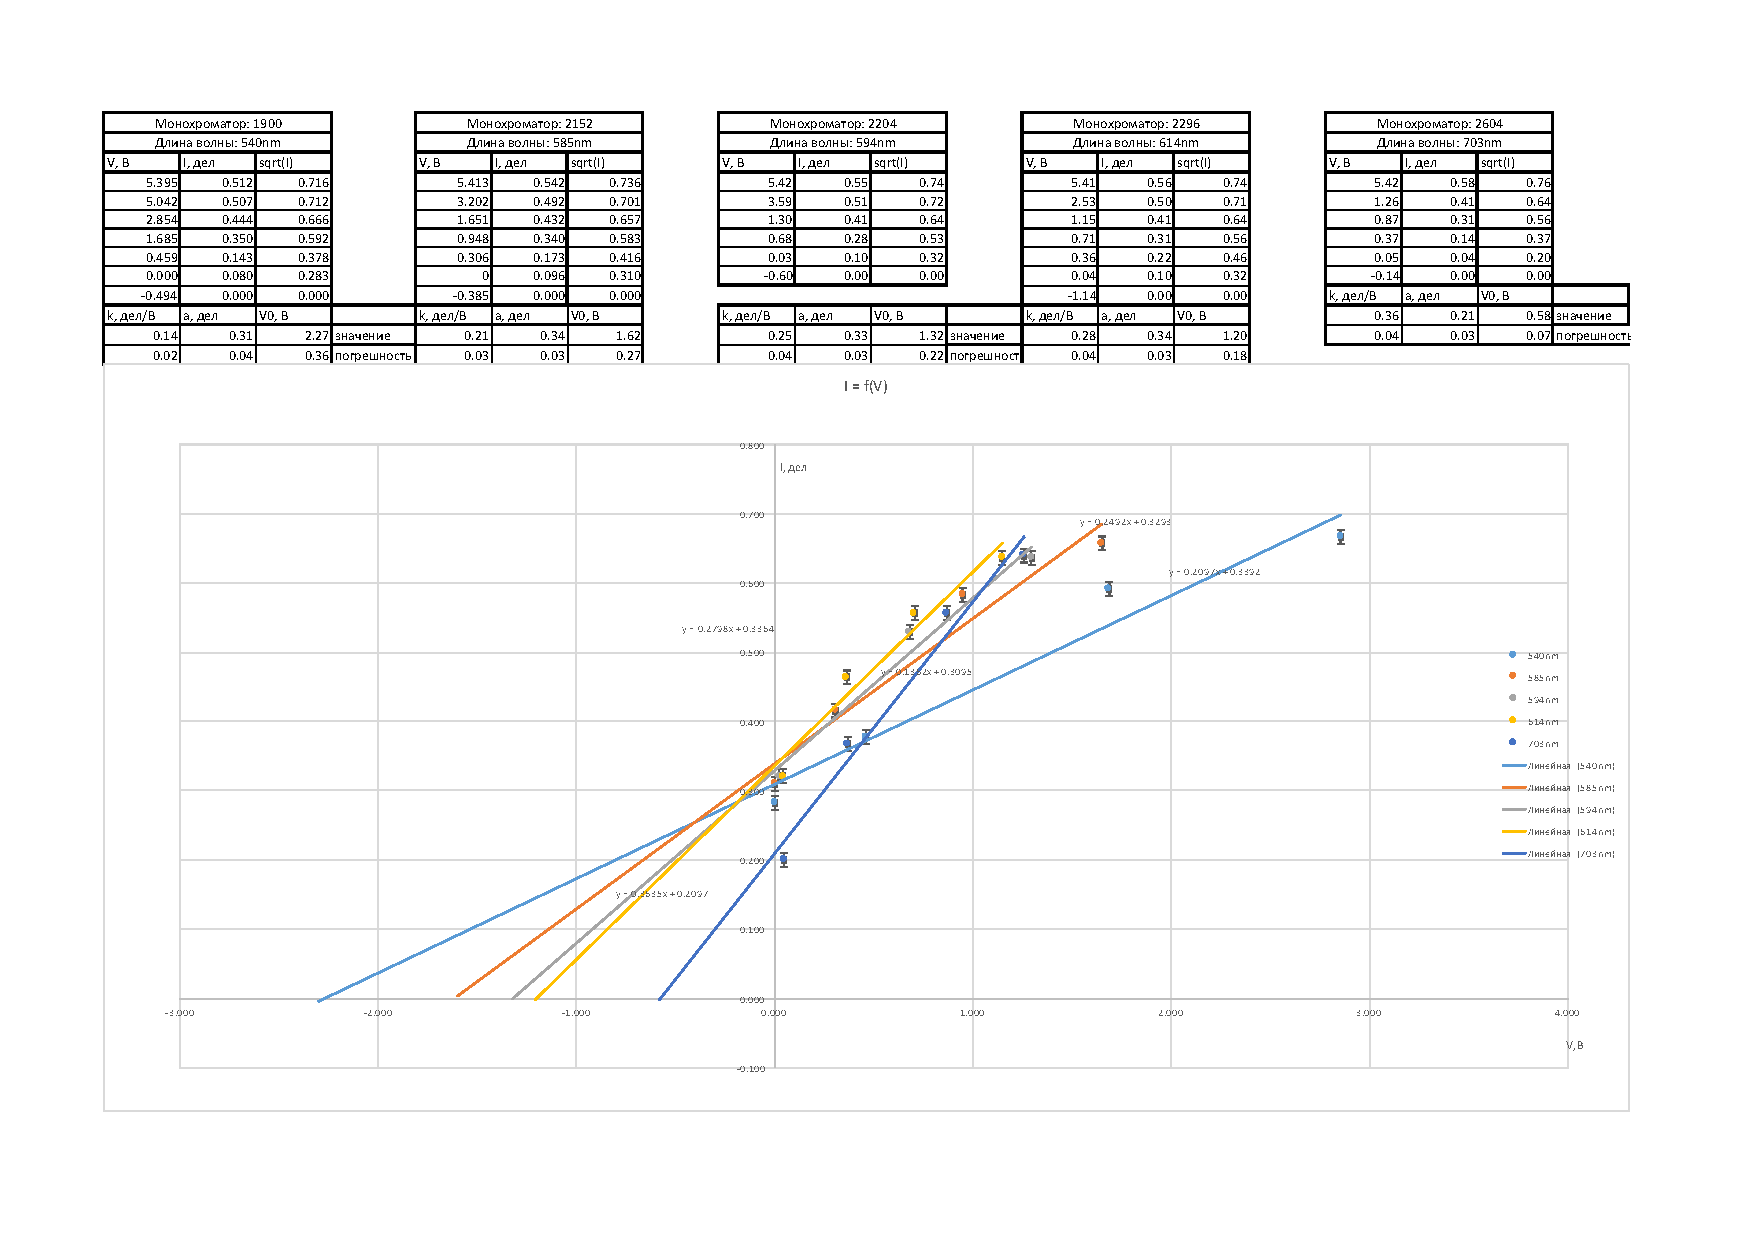
\includegraphics[width=\linewidth]{lab.pdf}}
\end{figure}

\item Вычисление $\frac{dV_0}{d\omega}$ и $\hbar$:

\begin{figure}[h]
 \center{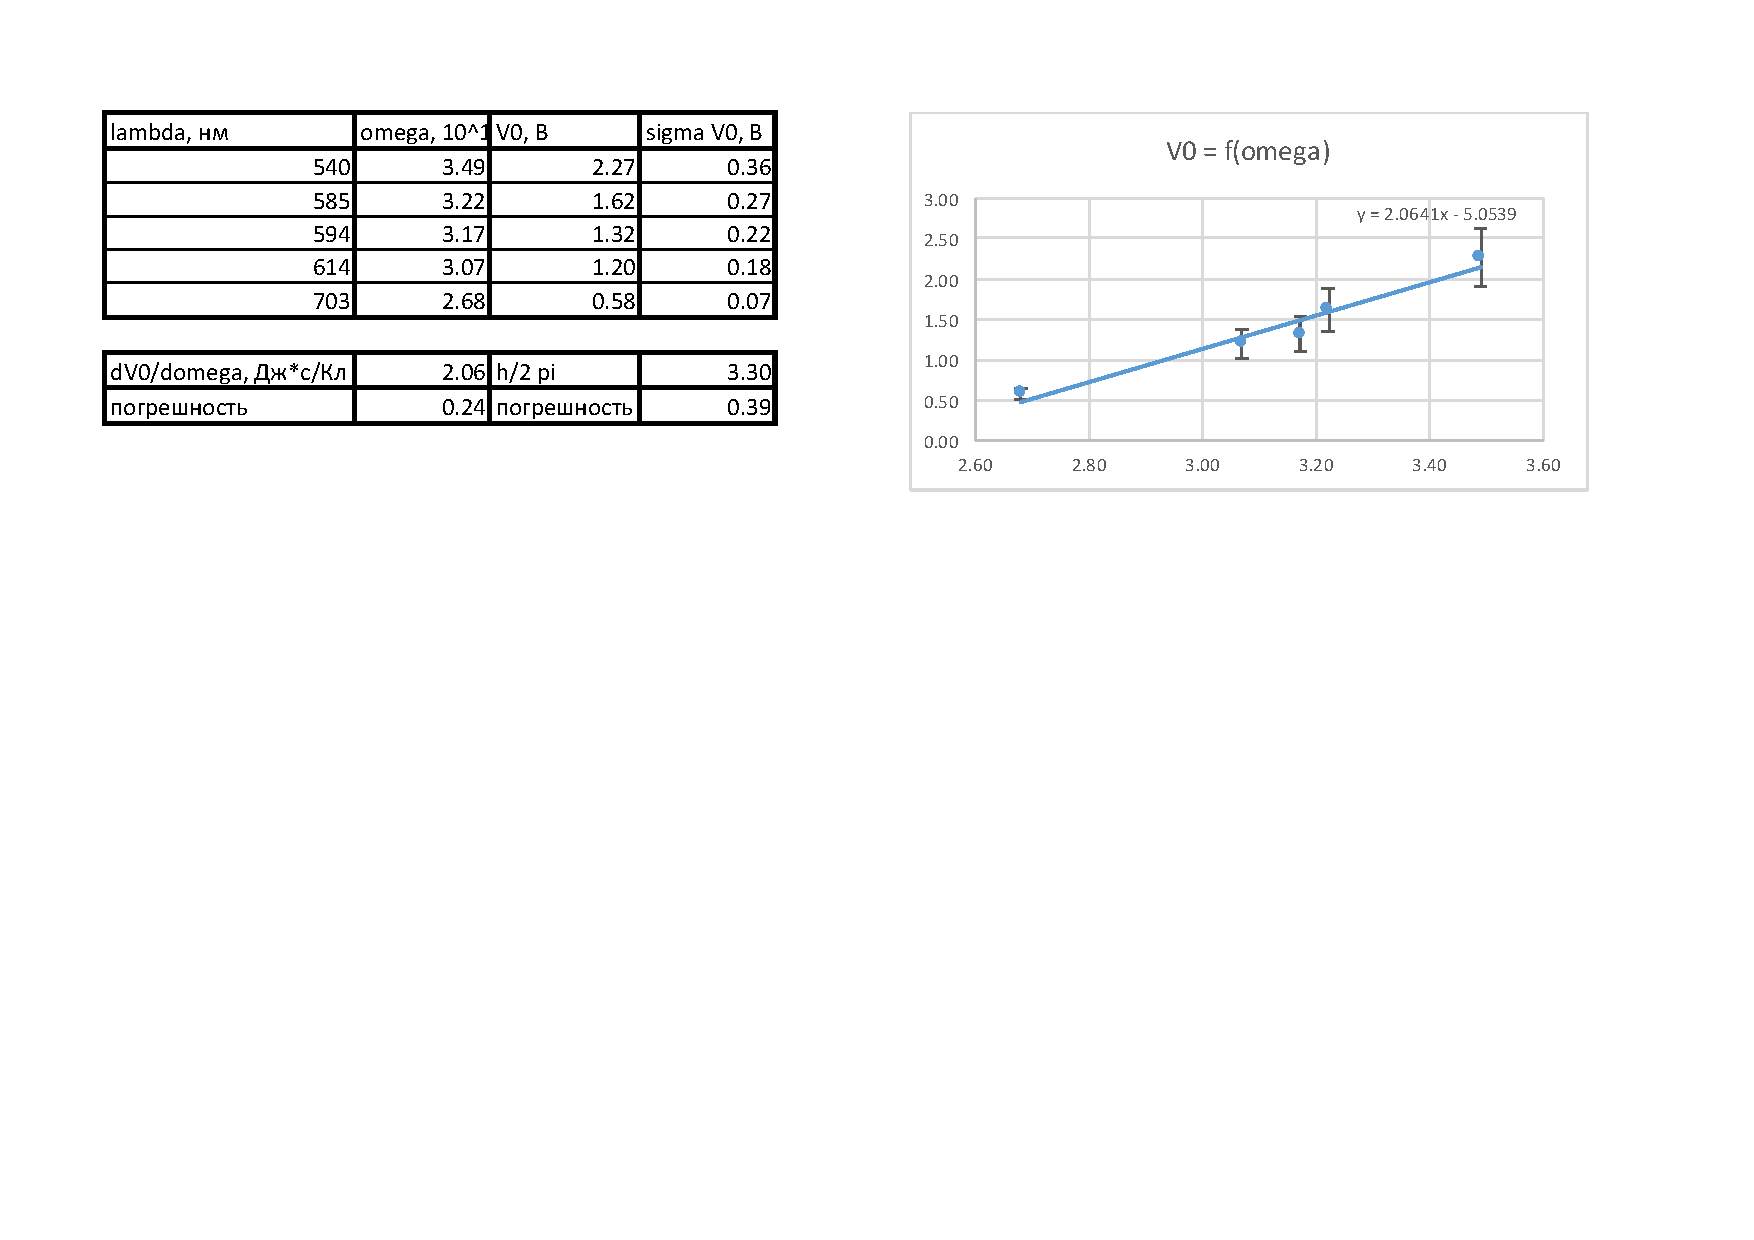
\includegraphics[width=.92\linewidth]{lab2.pdf}}
\end{figure}

\end{enumerate}

\section{Работа выхода и красная граница фотоэффекта}

Из графика следует, что $W \approx 5.05$ эВ. Красная граница фотоэффекта вычисляется из соотношения
\begin{equation}
\omega_{red} = \frac{W}{\hbar},
\end{equation}
и примерно равна $7.67 \cdot 10^{15} c^{-1}$.
\section{Вывод}

В ходе эксперимента подтвердились зависимости (\ref{einstein}) и (\ref{Idep}). Полученное значение постоянной Планка $(3.30  \pm 0.39 )\cdot 10^{-34}$ Дж $\cdot$ с отличается от табличного $\hbar = 1.05 \cdot 10^{-34}$ Дж $\cdot$ с примерно в три раза, но совпадает по порядку. Вероятная причина расхождения заключается в малом количестве экспериментальных данных. Наибольшая погрешность вносится большим временем установления напряжения на вольтметре.


\end{document}